\section{Theorical Background}

\subsection{Biến đổi Fourier Rời rạc (DFT)}
Trước khi thiết kế bộ FFT, cần xem xét định nghĩa gốc của Biến đổi Fourier Rời rạc (DFT). Với một tín hiệu đầu vào $x[n]$ có độ dài $N$, DFT được định nghĩa như sau:

\begin{equation}
	X[k] = \sum_{n=0}^{N-1} x[n] \cdot W_N^{kn}, \quad 0 \le k \le N-1
\end{equation}

Trong đó:
\begin{itemize}[label=-, leftmargin=2cm]
	\item $x[n]$: Chuỗi tín hiệu đầu vào miền thời gian.
	\item $X[k]$: Chuỗi tín hiệu đầu ra miền tần số.
	\item $W_N$: Hệ số quay (Twiddle Factor), được xác định bởi:
\end{itemize}

\begin{equation}
	W_N = e^{-j\frac{2\pi}{N}} = \cos\left(\frac{2\pi}{N}\right) - j\sin\left(\frac{2\pi}{N}\right)
\end{equation}

\textbf{Hạn chế của DFT trực tiếp:} Để tính toán trực tiếp, độ phức tạp thuật toán là $O(N^2)$. Với $N=8$, số phép nhân phức cần thực hiện là $8^2 = 64$. Điều này tiêu tốn nhiều tài nguyên phần cứng và làm giảm tốc độ xử lý.

\subsection{Thuật toán FFT (Cooley-Tukey Radix-2)}
Để tối ưu hóa phần cứng, thuật toán \textit{Cooley-Tukey Radix-2 Decimation-in-Time (DIT)} được sử dụng. Thuật toán này chia nhỏ bài toán DFT $N$ điểm thành hai bài toán DFT $N/2$ điểm (chẵn và lẻ) một cách đệ quy.

Công thức tổng quát cho Radix-2 DIT:
\begin{equation}
	X[k] = \text{DFT}_{N/2}\{x_{chan}\} + W_N^k \cdot \text{DFT}_{N/2}\{x_{le}\}
\end{equation}

Với thuật toán này, độ phức tạp giảm xuống còn $O(N \log_2 N)$. Đối với $N=8$, số tầng tính toán là $\log_2 8 = 3$ tầng, và tổng số phép tính cơ sở giảm đáng kể so với DFT truyền thống.

\subsection{Kiến trúc Tính toán Cơ sở}

\subsubsection{Đơn vị Cánh bướm (Butterfly Unit)}
Phần tử xử lý trung tâm của FFT Radix-2 là cấu trúc Butterfly. Một đơn vị Butterfly thực hiện tính toán trên hai mẫu đầu vào $A$ và $B$ để tạo ra hai mẫu đầu ra $A'$ và $B'$ theo công thức:
\begin{align}
	A' &= A + W_N^k \cdot B \\
	B' &= A - W_N^k \cdot B
\end{align}

Dưới đây là sơ đồ luồng tín hiệu của một đơn vị Butterfly:

\begin{figure}[h]
	\centering
	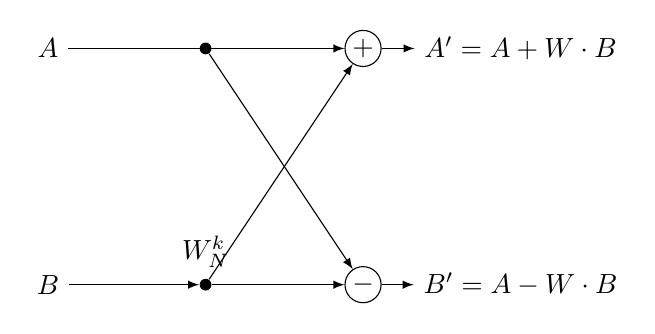
\begin{tikzpicture}[>=latex]
		% Nodes
		\node (A) at (0, 3) {$A$};
		\node (B) at (0, 0) {$B$};
		\node (Ap) at (6, 3) {$A' = A + W \cdot B$};
		\node (Bp) at (6, 0) {$B' = A - W \cdot B$};
		
		% Junctions
		\node[circle, fill, inner sep=1.5pt] (dot1) at (2, 3) {};
		\node[circle, fill, inner sep=1.5pt] (dot2) at (2, 0) {};
		\node (add) at (4, 3) [circle, draw, inner sep=1pt] {$+$};
		\node (sub) at (4, 0) [circle, draw, inner sep=1pt] {$-$};
		
		% Twiddle factor node
		\node (W) at (2, 0.1) [anchor=south] {$W_N^k$};
		\draw[->] (B) -- (dot2) node[midway, below] {}; 
		
		% Lines
		\draw[->] (A) -- (add);
		\draw[->] (dot1) -- (sub);
		
		\draw[->] (dot2) -- (add) node[pos=0.2, right] {};
		\draw[->] (dot2) -- (sub) node[pos=0.2, right] {};
		
		\draw[->] (add) -- (Ap);
		\draw[->] (sub) -- (Bp);
		
		% Annotation for multiplication
		%		\node at (2.8, 1.8) {$\times W_N^k$};
		
	\end{tikzpicture}
	\caption{Sơ đồ cấu trúc Butterfly Radix-2}
	\label{fig:butterfly}
\end{figure}

Về mặt phần cứng, mỗi Butterfly đòi hỏi:
\begin{itemize}[label=-]
	\item 1 Bộ nhân phức (Complex Multiplier).
	\item 2 Bộ cộng/trừ phức (Complex Adder/Subtractor).
\end{itemize}

\subsubsection{Đảo Bit (Bit Reversal)}
Do tính chất phân chia "Decimation-in-Time", đầu vào của bộ FFT cần được sắp xếp lại theo thứ tự đảo bit để đầu ra có thứ tự tự nhiên.
Ví dụ với $N=8$ (biểu diễn bằng 3 bit):
\begin{itemize}[label=-]
	\item Index $1$ ($001_2$) $\rightarrow$ Đổi thành $4$ ($100_2$).
	\item Index $3$ ($011_2$) $\rightarrow$ Đổi thành $6$ ($110_2$).
\end{itemize}
Trong thiết kế phần cứng, việc này thường được thực hiện bằng cách tráo đổi đường dây kết nối (hard-wired) ở tầng đầu vào, không tốn tài nguyên logic.

\subsection{Vấn đề Thực thi Phần cứng với Floating-Point}
Khác với Fixed-point, việc thiết kế FFT sử dụng Floating-point (thường theo chuẩn IEEE 754 Single Precision 32-bit) mang lại độ chính xác cao và dải động (dynamic range) lớn, nhưng đặt ra các thách thức thiết kế sau:

\begin{enumerate}
	\item \textbf{Định dạng dữ liệu (IEEE 754 Standard):} 
	Dữ liệu được biểu diễn dưới dạng $V = (-1)^S \times 1.M \times 2^{E-Bias}$.
	Mỗi số phức gồm 2 thanh ghi 32-bit (Phần thực và Phần ảo).
	
	\item \textbf{Độ phức tạp của khối tính toán:}
	\begin{itemize}
		\item \textit{Phép cộng/trừ:} Cần các khối logic cho việc so sánh số mũ, dịch bit để căn chỉnh phần định trị (alignment), cộng phần định trị, và dò tìm bit 1 đầu tiên (Leading One Detector) để chuẩn hóa lại.
		\item \textit{Phép nhân:} Cần nhân phần định trị và cộng số mũ, đồng thời xử lý tràn số (overflow/underflow).
	\end{itemize}
	
	\item \textbf{Độ trễ đường ống (Pipeline Latency):} 
	Do cấu trúc phức tạp của bộ cộng/nhân dấu phẩy động, mỗi phép tính thường mất nhiều chu kỳ xung nhịp (ví dụ: 3-5 cycles). Hệ thống cần thiết kế pipeline sâu để duy trì thông lượng (throughput) mà không làm giảm tần số hoạt động.
	
	\item \textbf{Lưu trữ Hệ số quay:} 
	Các giá trị $W_N$ được lưu trữ trong ROM dưới định dạng IEEE 754 32-bit.
\end{enumerate}
